\subsection{Surface Photometry for J1331 with MGEs}

%============================================================================

\begin{figure}
\centering
\includegraphics[width=0.8\columnwidth]{fig/1331F814Wsci_MGE_M.ps}
\caption{MGE for J1331's inner regions: Comparison of contours with constant F814W surface brightness of J1331's central region (orange lines) with the corresponding iso-brightness contours of the best fit MGE in table \ref{tab:MGEF814W}, convolved with the PSF in table \ref{tab:MGEF814W}, (gray lines). The MGE model is a good representation of the galaxy's light distribution within $\sim 5$ arcsec. Image scaling and orientation are indicated in the figure. The black line has a length of 10 arcsec and it's orientation corresponds to the galaxy's position angle as found in table \ref{tab:galaxyparameters}. For comparison the Einstein radius as found in table ??? is indicated as red dashed line. This MGE is used in the dynamical Jeans modelling in \S ???. [TO DO: explain how this MGE is used in dynamical modelling]}
\label{fig:MGEinnerRegions}
\end{figure}

\begin{figure}
\centering
\includegraphics[width=0.8\columnwidth]{fig/1331F814W_MGE_disk_L.ps}
\caption{MGE for J1331's outer regions: Comparison of contours with constant surface brightness of the smooth IRAF ELLIPSE model for J1331 in the F814W filter (yellow) with a corresponding best fit MGE (gray lines). The green box corresponds to the image section shown in Fig. \ref{fig:MGEinnerRegions}, with the Einstein radius as dashed red line. [TO DO: caption]}
\label{fig:MGEouterRegions}
\end{figure}

%============================================================================

\begin{table}
\centering
\caption{F814W PSF MGE: Parameters of the circular four-Gaussian MGE in Eq. (\ref{eq:PSFgeneral} fitted to the radial profile of the synthetic HST/F814W PSF image by [TO DO].}
\begin{tabular}{ccc}
\hline
$k$ & $G_k$ & $\delta_k$ [arcsec] \\\hline
1 & 0.184 & 0.038\\
2 & 0.485 & 0.085\\
3 & 0.222 & 0.169\\
4 & 0.109 & 0.487\\\hline
\end{tabular}
\label{tab:PSFMGEF814W}
\end{table}

\begin{table*}
\centering
\caption{J1331's F814W MGE: Parameters of the best fit MGE to the F814W surface brightness of J1331 in Fig. \ref{fig:F814W}. The fit is best inside an radius of 5 arcsec. The galaxy center and position angle, which gives the orientation of the MGE with respect to the original image, are given in table \ref{tab:galaxyparameters}. This MGE is used in the dynamical modelling in \S ???.  The first column gives the total F814W luminosity of the Gaussian in Eq. (\ref{eq:centralItotalL}) in units of counts. The second column is the corresponding I-band peak surface brightness in Eq. (\ref{eq:MGEgeneral}) in units of a luminosity surface density, calculated from the first column following the procedure described in \S ???. The third and fourth column give the dispersion and the last column the axis ratio of the Gaussian in Eq. (\ref{eq:MGEgeneral}).}
\begin{tabular}{cccccc}
\hline
 & total luminosity  & surface density & \multicolumn{2}{c}{Gaussian dispersion} & axis ratio\\
$k$  & $L_k$ [counts] & $I_{0,k}$ [$L_\odot$/pc$^2$] & $\sigma_k$ [arcsec] & $\sigma_k$ [kpc] & $q'_k$\\\hline
1  &     9425.96 &      20768.  &  0.051   & 0.103  & 1.00\\
2  &    13173.0 &        3161.2 &  0.178   & 0.358  & 0.76\\
3  &    40235.0 &        1588.2 &  0.503   & 1.008  & 0.58\\
4  &    67755.2 &         502.25&  1.180   & 2.368  & 0.56\\
5  &    203677. &         136.51&  3.891   & 7.805  & 0.57\\\hline
\end{tabular}
\label{tab:MGEF814W}
\end{table*}

%============================================================================

\begin{table*}
\centering
\caption{Galaxy Parameters of J1331}
\begin{tabular}{lllrl}
\hline
redshift                  & $z_d$ & 0.113 & \citep{SWELLSIII}\\
angular diameter distance & $D_d$ [Mpc] & 414 & \\
scaling                   & 1 kpc / 1 arcsec & 2.006 & \\
position angle            & $\phi$ [degrees] & wrt what???\\
average axis ratio & $q'$ & 0.598\\
average ellipticity & $\epsilon = 1 - q'$ & 0.402 & \\
apparent I-band magnitude & $m_\text{I}$ [mag] & 15.77 & \\
total I-band luminosity & $L_\text{tot,I}$ [$10^{10} L_\odot$] & 5.6 & \\
effective half-light radius & $R_\text{eff}$ [arcsec] & 2.6 & \\
& $R_\text{eff}$ [pc]& 5.2 & \\
\hline
\end{tabular}
\label{tab:galaxyparameters}
\end{table*}

%============================================================================

In \S ??? we derived a mass model for J1331 from Lensing. In this section set up a model for the galaxy's intrinsic light distribution in terms of an MGE, which we will then compare to the mass distribution. The light model will also be the basis of the dynamical Jeans modelling in \S ???.
\\To derive J1331's surface brightness distribution, we use the HST image in the infrared F814W filter, shown in Fig. \ref{fig:F814W}. In infrared J1331's central old and smooth stellar component is more extended than in the F450W filter in Fig. \ref{fig:F450W}, which is more sensitive to young clumpy star-forming regions. In infrared the bulge is also much brighter than the bluish lens images and the imaging is less prone to extinction. The F814W image is therefore best suited for fitting a MGE. 

\paragraph{PSF for the HST/F814W filter.} We find a radial profile for the HST/F814W filter PSF from circular annuli within a synthetic PSF image from [TO DO: Where did we get this image from???], ignoring diffraction spikes. The one-dimensional MGE fit of Eq. (\ref{eq:PSFgeneral}) to this radial profile is performed using the code by [TO DO: REF and footnote to code]. The MGE parameters of the normalized PSF model are given in Tab. \ref{tab:PSFMGEF814W}.

\paragraph{MGE for the inner regions.} We fit a MGE to the smooth central region within radius $\sim 5$ arcsec of the HST/WFPC2/WF3/F814W image of J1331 in Fig. \ref{fig:F814W}. Bright objects  close to the galaxy, blobs possibly belonging to the background galaxy and parts of the foreground spiral arm were masked during the fit. J1331's galaxy center, position angle and average apparent ellipticity (see table \ref{tab:galaxyparameters}) are found from the images weighted first and second moment. The MGE fit, as performed by the code \cite{Cap02}, splits the image in annuli with the given ellipticity and position angle and sectors of $5^\circ$ width and fits an 5-Gaussian MGE of the form in Eq. (\ref{eq:MGEgeneral}) convolved with the PSF MGE in table \ref{tab:PSFMGEF814W} to it. The best fit MGE (PSF convolved) is compared to the data in Fig. \ref{fig:MGEinnerRegions} and the corresponding parameters of the intrinsic surface brightness distribution are given in table \ref{tab:MGEF814W}. The fit is a very good representation of the light distribution in the inner 5 arcsec, but underestimates the light distribution outside of this.

\paragraph{MGE for the outer regions.} To get an handle on the light distribution also in the outer parts of J1331, where spiral arms dominate, we first fit a IRAF ELLIPSE [TO DO: How to reference???] model to the F814W image (masking the brightest blobs in the spiral arms and outer regions). Only then we fit a 7-Gaussian MGE to the smooth ellipse model. The MGE does not perfectly reproduce the flattness of the ellipse model at every radius, but considering the spiral arm dominated outer regions of J1331, it is good enough for an approximate handling of the overall light distribution.

\paragraph{Transformation into physical units.} To transform the MGE in units of counts into physical units, we apply a simplified version of the procedure described in \citet{Holtzman}, analogous to [TO DO: Cappellari Read me file???]
\\The scaling of the drizzled HST/WFC3 images is  $S = 0.05$ arcsec/pixel and the total exposure time $T = 1600$ sec. The total F814W luminosity in counts of each Gaussian of the MGE has a central surface brightness in counts per pixel of
\begin{equation*}
C_0\text{[counts/pixel]} = \frac{L[\text{counts}]}{2\pi \sigma[\text{pixel}]^2 q}.
\end{equation*}
This is then transformed into an I-band surface brightness via
\begin{equation}
\mu_I \simeq -2.5 \log_{10}\left( \frac{C_0\text{[counts/pixel]}}{T[\text{sec}] \cdot S[\text{arcsec/pixel}]^2}\right) + Z + C + A_I, \label{eq:muI_}
\end{equation}
where $Z\simeq21.62$ is a the zero-point from \citet{Holtzman}  (updated according to \citet{Dolphin,DolphinNew}) for the photometric system of the HST/WFPC2 camera and the F814W filter plus a correction for the difference in gain between calibration and observation. $C= 0.1$ corrects for the finite aperture of the WFPC2. And $A_I =0.015$ mag  is the extinction in the I-band tpwards J1331, according to the NASA/IPAC Extragalactic Database [TO DO: proper reference]. The color-dependent correction between the F814W filter and the I-band of the UBVRI photometric system is  small \citep{Holtzman} and we neglect it therefore. The last step is to transform the surface brightness $\mu_i$ in mag to the I-band surface density of the Gaussian in $L_\odot$/pc$^2$ as
\begin{eqnarray*}
I_0[L_\odot \text{pc}^{-2}] = \left( 64800/\pi\right)^2 \left(1+z \right)^4 10^{0.4\left(M_{\odot,I}-\mu_I \right)},
\end{eqnarray*}
where the term with $z$ accounts for redshift dimming and $M_{\odot,I}=4.08$ mag is the sun's absolute I-band magnitude \citep{1998gaas.book.....B}. The luminosity $L_k$[counts] and the corresponding surface brightness density $I \equiv I_{0,k}[L_\odot \text{pc}^{-2}]$ of each Gaussian are given in Table \ref{fig:MGEinnerRegions}. [TO DO: I'm really confused about this. Check, that everything is correct and the naming of quantities, e.g. with or without subscripts of 0, is fine???] [TO DO: Maybe shift to appendix???]

\paragraph{Inclination.} [TO DO: Do we need this for the dynamical modelling???? Is described on p. 56]

\paragraph{Total luminosity and effective radius.} J1331's total I-band luminosity is easily determined by summing up the luminosity contributions of all the Gaussians of the MGE for the outer regions (shown as gray lines in Fig. \ref{fig:MGEouterRegions}). We find $L_\text{tot,I} \simeq 5.6 \cdot 10^{10} L_\odot$. This corresponds to an apparent magnitude of $m_I = 15.77$ mag. We determine the circularized effective radius $R_\text{eff}$ of J1331 from the definition $L(<R_\text{eff}) \equiv \frac 12 L_\text{tot}$ and the growth curve $L(<R)$ from the MGE model of the outer regions [TO DO: Maybe I need a table anyway???], where $R$ is the projected radius on the sky [TO DO: Or is it $R'$???]. We find the effective radius to be $R_\text{eff} \simeq 2.6 \text{arcsec} \hat{=} 5.2 \text{kpc}$.  All values are summarized in Table \ref{tab:galaxyparameters}.



\paragraph{[TO DO: Stuff to mention]}
\begin{itemize}
\item the deporjecten if the galaxy under the assumption of oblate axisymmetry and an estimated inclination of $\sim70^\circ$ can be performed analytically.
\end{itemize}


